\section{Preprocesado de datos}

Tomaremos como ejemplo la base de datos \emph{movieslens}\footnote{\url{<http://grouplens.org/datasets/>}}, publicada en \cite{MovieLens}. Esta base de datos describe la calificación de 5 estrellas un servicio de recomendación de películas. Contiene 100836 clasificaciones en 9742 películas. Estos datos fueron creados por 610 usuarios entre el 29 de marzo de 1996 y el 24 de septiembre de 2018. Este conjunto de datos se generó el 26 de septiembre de 2018. Todos los usuarios seleccionados habían calificado al menos 20 películas. 

A continuación explicaremos los pasos realizados para la obtención del historial de usuario, y luego explicaremos como agregaremos información para que sea posible el analisis de un sistema de recomendación


\subsection{Descripción de la base de datos}


Los datos están contenidos en las bases de datos: 
\begin{itemize}
    \item \textbf{movies.csv}: base de datos donde se describe enlaza el identiciador numético de la película con el nombre y los generos a los que pertenece. A continuación se describe las variables de esta base de datos:
    \begin{center}
        \begin{tabular}{|c|c|c|c|c|}
        \hline
        \textbf{Variable} & \textbf{Descripción} & \textbf{Tipo} & \textbf{Ejemplo 1} & \textbf{Ejemplo 2} \\ 
        \hline
         movieId & identificador & numérico & 1 & 3431 \\  
         title & nombre  & string & 
                Toy Story (1995)  & 
                Braveheart (1995)    \\
         genres & generos  & string & Comedy|Horror & Comedy|Drama|Romance \\
         \hline
        \end{tabular}
    \end{center} 
    \item \textbf{ratings.csv}: base de datos donde se registra para cada usuario y cada película que ha visto, la puntación que ha dado. A continuación se describe las variables de esta base de datos:
    \begin{center}
        \begin{tabular}{|c|c|c|c|c|}
        \hline
        \textbf{Variable} & \textbf{Descripción} & \textbf{Tipo} & \textbf{Ejemplo 1} & \textbf{Ejemplo 2} \\ 
        \hline
         userId & identificador de usuario   & numérico & 311 & 3431 \\  
        %
         movieId & identificador de película & numérico & 54 & 23 \\
        %
         rating & puntación  & numérico & 3 & 5 \\
        %
        timestamp & instante de tiempo  & numérico & 964983815 & 864913515 \\        
         \hline
        \end{tabular}
    \end{center} 
\end{itemize}

Dado que queremos ver una recuerencia en el comportamiento de los usuario es muy dificil predecir las películas de manera indivudual. Podemos preguntarnos cuantas veces el usuario va a volver a mirar la misma película. Dado que la respuesta es muy pocas, los datos de entrenamiento para la predicción de la pélicula serán muy pequeñas. Si pensamos en una película como un elemento perteneciente a un espacio vectorial de caráterísticas podemos tener más datos de entrenamiento. 

Para ello, cruzaremos la base de datos \emph{movies.csv} y \emph{rating.csv}, para crear una nueva base de datos que en sus variables contenga cada uno de los generos disponibles en la totalidad de los datos. 



\begin{center}
    \begin{tabular}{|c|c|c|c|c|}
    \hline
    \textbf{Variable} & \textbf{Descripción} & \textbf{Tipo} & \textbf{Ejemplo 1} & \textbf{Ejemplo 2} \\ 
    \hline
     userId & identificador de usuario   & numérico & 311 & 3431 \\  
    %
     rating & puntación  & numérico & 3 & 5 \\
    %
    timestamp & instante de tiempo  & numérico & 964983815 & 864913515 \\        
    \hline
    %
     comedy & ¿pertenece a comedy?  & boleano & 0 & 1 \\  
    %
     Drama & ¿pertenece a Drama?  & boleano & 0 & 1 \\  
    %
    Horror & ¿pertenece a Horror?  & boleano & 0 & 1 \\  
    %
    \dots & \dots  & \dots & \dots & \dots  \\  
        %
    \dots & \dots  & \dots & \dots & \dots  \\  
     \hline
    \end{tabular}
\end{center} 


Si consideramos que tenemos $d$ géneros, entonces para cada usuario tenemos una secuencia de vectores $\bm{x}_t \in [0,1]^d \ | \ \forall t \in \{ 1,\dots,T\}$. Por último, si una película pertenece a varios géneros a la vez, el módulo del vector asociado será más grande que una película con menos géneros asociados. Dado que el módulo de un vector puede afectar a los modelos de prodicción normalizaremos todos los vectores $\bm{x}_d$. 

Asi pues, el historial de un usuario se puede entender como la rotación de un vector $\bm{x}_t$:

\begin{gather}
    \{ \bm{x}_t  \}_{t \geq0} \in \mathbb{R}^d \ \ | \ ||\bm{x}_t|| = 1 \ \forall t \leq 0
\end{gather}

\subsection{Generación del historial de recomendación ficticio}

El problema que tenemos en estos datos es que solo tenemos las películas que el usuario ha seleccionado en cada iteración, sin embago si consideramos el proceso de recomendación en cada iteración el usuario se le ha recomendado una serie de peliculas de las cuales solo tenemos constancia la película que ha seleccionado. Es por ello que consideraremos que en cada iteración el sistema de recomendación a ofrecido dos películas al usuario. Una de ella la ha aceptado y la otra la ha rechazado. Para crear el historial de películas rechazadas agregaremos de manera ficticia otra película que tengamos en el historial del usuario pero que tenga menor puntación que la película que ha selecionado en la realidad. En los cuadros \ref{cuadroacp} y \ref{cuadrorec} se muestran dos ejemplos del historial de acetación y de rechazo respectivamente. 

\begin{obs}
    Para el historial de aceptación tambien tenemos su correspondiente puntación, sin embargo para el historial de rechazos dado que el usuario no lo ha selecionado, en general no tenemos puntación asociada.
\end{obs}
\begin{table}
\begin{center}
    \begin{tabular}{|c|c|c|c|c|c|c|}
        \hline
        \textbf{title}          &              \textbf{rating}  &  \textbf{timestamp}   &    \textbf{Action}   &  \textbf{Adventure} & \dots \\
        \hline
"Shawshank Redemption, The (1994)"    &     3    &  1.4795e+09      &  0    &    0 & \dots\\
"Fight Club (1999)"                   &     5    &  1.4795e+09      &  0.5  &    0 & \dots\\
"Face/Off (1997)"                     &   3.5    &  1.4795e+09      &  0.5  &    0 & \dots\\
"Paycheck (2003)"                     &   1.5    &  1.4795e+09      &  0.57735  &         0 & \dots\\
"Mission: Impossible II (2000)"       &    3     &  1.4795e+09      &  0.57735  &   0.57735 & \dots\\
"Broken Arrow (1996)"                 &   3.5    &  1.4795e+09      &  0.57735  &   0.57735 & \dots\\
"Windtalkers (2002)"                  &     3    &  1.4795e+09      &  0.57735  &         0 & \dots\\
\hline
    \end{tabular}
\end{center}
\caption{Ejemplo de historial de aceptación de un usuario}\label{cuadroacp}

    
\begin{center}
    \begin{tabular}{|c|c|c|c|c|c|c|}
\hline
\textbf{title}          &              \textbf{rating}  &  \textbf{timestamp}   &    \textbf{Action}   &  \textbf{Adventure} & \dots \\
\hline
"The Drop (2014)"                   &      2   &   1.4795e+09  &       0        & 0  & \dots \\  
"Django Unchained (2012)"           &    3.5   &   1.4795e+09  &       0.57735  & 0  & \dots \\ 
"Interstellar (2014)"               &      3   &   1.4795e+09  &       0        & 0  & \dots \\  
"The Drop (2014)"                   &      2   &   1.4795e+09  &       0        & 0  & \dots \\  
"The Drop (2014)"                   &      2   &   1.4795e+09  &       0        & 0  & \dots \\  
"Exit Through the Gift Shop (2010)" &      3   &   1.4795e+09  &       0        & 0  & \dots \\  
"Collateral (2004)"                 &    3.5   &   1.4795e+09  &       0.5      & 0  & \dots \\  
    \hline
    \end{tabular}
\end{center}
\caption{Ejemplo de historial de rechazos de un usuario}\label{cuadrorec}
\end{table}



De esta manera tenemos para cada usuario:

\begin{itemize}
    \item el historial de películas aceptadas, que denotaremos como: $\{\bm{x}^a_t\}_{t\geq 0}$ 
    \item el historial de rechazadas, que denotaremos como: $\{\bm{x}^r_t \}_{t\geq 0}$
\end{itemize} 


\section{Espacios de estados, acciones y recompensas}

Definimos una proceso de deción de Markov inspirado en \cite{shani2005mdp}
\begin{itemize}
    \item \textbf{Estado}: Pelicula vista en el instante anterior. Representado por $\bm{x}_{t} \in \Ss = \mathbb{R}^d$, donde $d$ es el número de generos considerados en la base de datos. 
    \item \textbf{Acción}: Las dos películas que enseñamos al usuario. Entonces la acción viene representado por  $\bm{a}_t \in \As = \mathbb{R}^d \times \mathbb{R}^d$. 
    \item \textbf{Recompenza}: Puntación que da a la película selecionada. Representado por $r_t \in \{1,2,3,4,5\}$. Suponemos que este puede depender del estado $\bm{x}_t$ y de la acción $\bm{a}_t$, sin embargo no sabemos que forma funcional tiene.
    \item \textbf{Ecuación dinámica}: Tal como se ha creado la base de datos, sugiere que la dinámica del usuario puede escoger la película según la puntación asociada. Sin embargo, en el plantamiento el usuario hasta despues de ver la película no tiene una puntación asociada por lo que la puntación a \emph{priori} que tiene el usuario sobre dos películas es la que determina la eleción. Dado que en la metodología de aprendizaje por refuerzo no es necesario el conocimiento de la dinámica, no es necearia definirla.
\end{itemize}

Mostramos un esquema de la interación del usuario y el sistema de recomendación en la figura \ref{sqmrs}

\begin{obs}
    La acción en cada instante $t$ es un par de vectores $\bm{x}_1,\bm{x}_2 \in \mathbb{R}^d$, sin embargo en la realidad el sistema de recomendación deberá recomendar un título de película y no un vector de caráterísticas. Por esta razón, necesitamos una función que traduzca un vector de caráterísticas $\bm{x}$ en un titulo de la base de datos. Tomaremos como peliculas correspondiente a $\bm{x}$ la película más parecidad que tengamos en la base de datos y que no haya visto el usuario.
\end{obs}




\tikzstyle{startstop} = [rectangle, rounded corners, minimum width=2cm, minimum height=1cm,text centered, draw=black, fill=blue!30,line width=1.25pt]
\tikzstyle{cir} = [circle, rounded corners, minimum width=1.5cm, minimum height=1cm,text centered, draw=black, fill=green!30,line width=1.25pt]
\tikzstyle{cir_hd} = [circle, rounded corners, minimum width=1.5cm, minimum height=1cm,text centered, draw=black, fill=red!30,line width=1.25pt]
%%%%%%%%%%%%%%%%%%%%%%%%%%%%%%%%%%%%%%%%%%%%%%%
% for double arrows a la chef
% adapt line thickness and line width, if needed
\tikzstyle{vecArrow} = [thick, decoration={markings,mark=at position
   1 with {\arrow[semithick]{open triangle 60}}},
   double distance=1.4pt, shorten >= 5.5pt,
   preaction = {decorate},
   postaction = {draw,line width=2.4pt, white,shorten >= 4.5pt}]
\tikzstyle{innerWhite} = [semithick, white,line width=1.4pt, shorten >= 4.5pt]

\begin{figure}[]
    \centering

    \begin{tikzpicture}[node distance=3cm]
        \filldraw[color=red!60, fill=red!5, very thick](8.5,1.2) rectangle (3,-7.5);
        \node[draw] at (7.65,0.85) {\textbf{Agente}};


        \node (start) [startstop] {Usuario};
        \node (state) [cir,above right of=start] {$\bm{x}_{t-1}$};
        \node (action) [cir,below right of=state] {$\bm{a}_{t}$};
        \node (reward) [cir,below right of=start] {$r_{t}$};
        \node (nextstate) [cir,below left of=start,] {$\bm{x}_{t}$};

        \node (RS) [startstop,below right of=reward] {$Sis. \ Rec.$}; 

        %
        \node (m2) [cir_hd,below right of=RS] {$\text{película}_{2}$};
        \node (m1) [cir_hd,above right of=RS] {$\text{película}_{1}$};
        %
        \draw  [line width=1.25pt,bend left=-70,<-] (state) edge (nextstate);
        \draw  [line width=1.25pt,bend left=-30,<-] (start) edge (state);
        \draw  [line width=1.25pt,bend left=-35,<-] (nextstate) edge (start);
        \draw  [line width=1.25pt,<-] (start) edge (action);
        \draw  [line width=1.25pt,bend left=35,<-] (reward) edge (start);
        %
        \draw  [line width=1.25pt,bend left=-35,<-] (action) edge (m1);
        \draw  [line width=1.25pt,bend left=85,<-] (action) edge (m2);
        %
        \draw  [line width=1.25pt,bend left=45,<-] (m1) edge (RS);
        \draw  [line width=1.25pt,bend left=-45,<-] (m2) edge (RS);
        %
        %
        \draw  [line width=1.25pt,bend left=70,<-] (RS) edge (nextstate);
        \draw  [line width=1.25pt,bend left=40,<-] (RS) edge (reward);


    \end{tikzpicture}
    \caption{Esquema de la interacción del sistema de recomendación y el usuario}
    \label{sqmrs}

    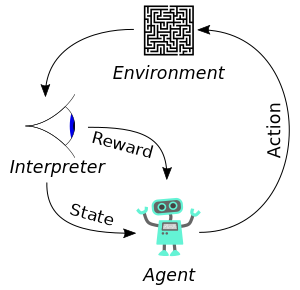
\includegraphics[scale=1]{img/Reinforcement_learning_diagram.png}
    \caption{Esquema estándar del aprendizaje por refuerzo \cite{WikiRF}}

\end{figure}



\section{Plantamiento de los problemas}

En esta tesis buscarémos políticas para realizar buenas recomendaciones de manreda que la puntación acumuladad del usuario sea máxima. Este problema puede ser planteado desde el momento en el que el usuario empieza a usar el sistema de recomendación o cuando tenemos ya historial suficiente del usuario para poder inferir una manera de actuar. En el primero de ellos, dado que no tenemos ninguna información del usuario deberemos utilizar los datos de los usuarios anteriores. Acontinuación plantemos los dos problemas.

\begin{problem}\label{prob1}
    Suponiendo que tenemos un base de datos de historial de aceptación $\{ \bm{x}_t^a\}_{t\geq 0}$ y rechazo de varios usuarios $\{ \bm{x}_t^r\}_{t\geq 0}$ ¿Cómo podemos obtener una política $\pi: \Ss \rightarrow \As $, que nos maximize la recompensa acumulada?
\end{problem}

\begin{problem}\label{prob2}
    Suponiendo que tenemos un historial de aceptación $\{ \bm{x}_t^a\}_{t\geq 0}$ y de rechazo $\{ \bm{x}_t^r\}_{t\geq 0}$ del usuario. ¿Cómo podemos obtener una política $\pi: \Ss \rightarrow \As $ que nos maximize la recompensa acumulada?
\end{problem}






\section{Metodología}


\subsection{Seleción de estado inicial}

Dado que la condición incial se determina por una primera recomendación que no nos es posible determinar lo tomaremos como aleatorio. Luego buscaremos la política óptima que nos permita encontrar los datos de entrenamiento. 

\subsection{Obtención de la política para el problema (\ref{prob1})}

\subsection{Obtención de la política para el problema (\ref{prob2})}
En cierto momento tenemos un historial de usuario, hacemos \emph{Q-learning} mediante las acciones que tenemos disponibles. En \cite{fujimoto2019off}, se estudia el problema de aprendizaje por refuerzo cuando tenenemos los datos ya dados. Alli se ve que la convergencia del algoritmo \emph{Q-learning} dentro de un conjunto de datos ya dados tambien converge a la política óptima.

\begin{thm}
    \cite{fujimoto2019off}. \textit{La realización de Q-learning mediante el muestreo de un conjunto de datos $B$ converge a la función valor óptimo.}
\end{thm}

Entonces 
\begin{gather}
    Q(s,a) \leftarrow (1-\alpha)Q(s,a) + \alpha \bigg( r +\gamma \max_{a' s.t (s',a') \in \mathcal{B}} Q(s',a') \bigg)
\end{gather}

\begin{algorithm}[!ht]
    \caption{\emph{Batch Q-learning }}\label{Qlearning}
    \begin{algorithmic}[1]
        \Procedure{Bacth Q-learning}{$\mathcal{Q}^{*},s_0,tol,\alpha,\epsilon$}
        \State $k \gets 0$
        \State $\mathcal{Q}_1 \gets \mathcal{Q}^{*}$
        \While{$ error \leq tol$}
            \State $k \leftarrow k + 1$
            \State Sample $(s_t,a_t,s_{t+1},r_t)$
            \State $\displaystyle \mathcal{Q}_k(s_t,a_t) \gets (1-\alpha)\mathcal{Q}_{k-1}(s_t,a_t) +  
            \big[ r_t + \gamma \max_{a'\in \As \ s.t.(s_{t+1},a')  \in \mathcal{B} \ }\mathcal{Q}_{k-1}(s_{t+1},a') \big]$
            \State $error=|| Q_k - Q_{k+1}||^2$

        \EndWhile
        \State \textbf{return} $\{a_t\}_{t>0}$
        \EndProcedure
    \end{algorithmic}
\end{algorithm}


La evaluación de la política se realizará mediante el uso de los datos restantes. Para ello se selecionará la acción óptima como la acción que nos mande la política encontrada, proyectado a los datos que tengamos en los datos restantes.



\subsection{Evaluación de las políticas}

Dado que no podemos simular el comportamiento del usuario lo que haremos es escoger un proyección la película recomendada al historial de prueba, es decir las dos películas que el sistema tiene que recomendar se selecionará del historial de prueba de manera que sea la más cercana medida en la distancai euclidea a la película que mande la política. 

\section{Resultados numéricos}

